% fuentes de esta seccion 
% https://www.mdpi.com/2076-3417/12/5/2606
% https://tesis.ipn.mx/jspui/bitstream/123456789/18688/1/Sistema%20de%20control%20para%20el%20desplazamiento%20omnidireccional%20de%20un%20robot%20m%C3%B3vil.pdf


\subsubsection{Modelo cinemático}

La cinemática se define como la ciencia que estudia el movimiento de objetos sin tomar en cuenta sus inercias. Dentro de la misma se estudia la posición, la velocidad, la aceleración y todas las demás derivadas de alto orden de las variables de posición con respecto al tiempo.

Para lograr representar matemáticamente al robot se utilizan ecuaciones que relacionan las velocidades de las ruedas con la velocidad lineal y angular del robot en el plano. Estas ecuaciones se derivan de la disposición geométrica de las ruedas y las características de las ruedas omnidireccionales. Utilizando matrices de transformación, es posible describir cómo las velocidades de las ruedas se combinan para producir el movimiento deseado del robot. Para ello se definen dos elementos fundamentales, la ecuación cinemática directa y la ecuación cinemática inversa. \cite{tzafestas2013introduction}

En el contexto de un robot omnidireccional de 4 ruedas, la cinemática directa permite traducir un vector de movimiento lineal del robot en velocidades específicas para cada rueda independiente. Cada rueda se mueve independientemente y por su configuración, permite que el robot se pueda desplazar lateralmente, hacia adelante, hacia atrás, gire sobre su propio eje y realice trayectorias curvas. \cite{rijalusalamkinematics}

Es importante que tengamos en cuenta que para tener un sistema de control acotado y predecible, es necesario compensarlo de algún modo. En este caso debemos ser capaces de obtener el vector de movimiento del robot en base a las velocidades angulares medidas en las ruedas y así lograr detectar diferencias con el vector de movimiento deseado. Para ello nos resulta útil la cinemática inversa, que implica medir las velocidades angulares de cada una de las cuatro ruedas para obtener el vector de movimiento que el robot realiza. Esto es crucial para el control y navegación del robot dado que corrige las alteraciones de un entorno dinámico.

El desarrollo de estas ecuaciones implica calcular cómo las velocidades de cada rueda contribuyen al movimiento global del robot y cómo se deben ajustar estas velocidades para lograr una trayectoria específica. En otras palabras, estas ecuaciones toman en cuenta la disposición y orientación de las ruedas y cómo contribuyen al movimiento global del robot, aprovechando al máximo la capacidad omnidireccional del robot.

Una vez logrado un modelo cinemático que aproxime bien el sistema real, deberíamos poder establecer un vector de movimiento deseado y obtener la velocidad a la que se debe colocar cada rueda para poder transcurrirlo. No solo debería poder hacer movimientos rectos en cualquier dirección, sino que también sería capaz de hacer movimientos rotatorios con traslación sobre el plano, formando trayectorias elípticas. \cite{rijalusalamkinematics}

En nuestro caso se trata de un robot cuadrado con 1 rueda por cada lado cuya orientación respecto al robot es fija. Ademas de ello, se utilizan ruedas de tipo Omni-wheel, las cuales son similares a las ruedas Mecanum. Son ruedas que cuentan con pequeños discos (llamados rodillos) alrededor de la circunferencia perpendiculares a la dirección de giro. El efecto es que la rueda puede moverse con toda su fuerza, pero también se deslizará lateralmente con gran facilidad.

\begin{figure}[H]
    \centering
    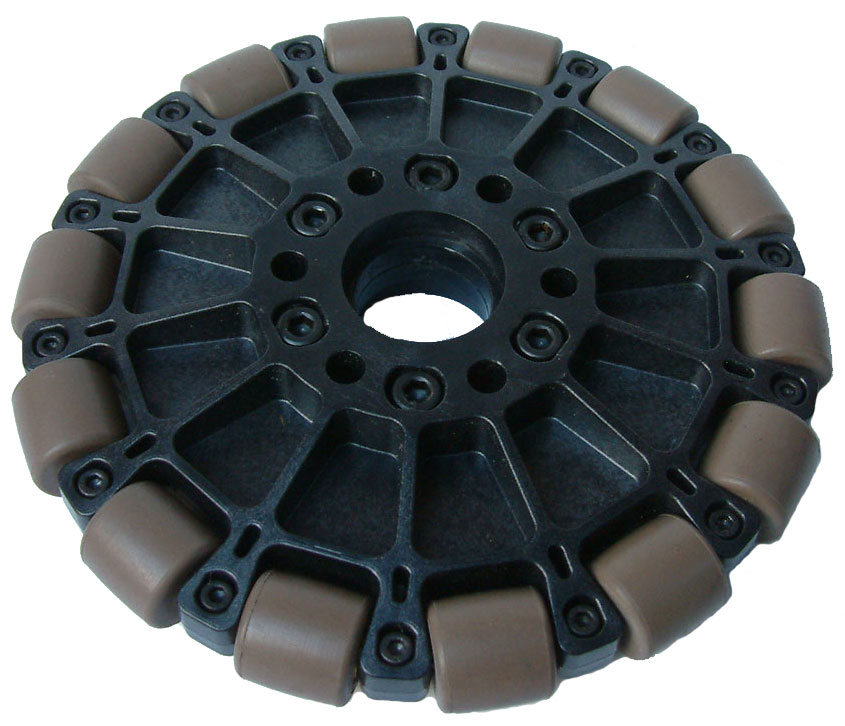
\includegraphics[width=0.3\linewidth]{omni-wheel-wikipedia}
    \caption{Rueda omnidireccional Omni-Wheel}
    \label{fig:ruedaomniwheel}
\end{figure}

Teniendo en cuenta lo anterior, para la construcción del modelo cinemático se consideran las siguientes limitaciones:

\begin{itemize}
    \item El robot se mueve sobre una superficie plana lisa.
    \item No existen elementos flexibles en la estructura del robot.
    \item El eje de direccionamiento de las ruedas siempre es perpendicular al suelo.
    \item No se consideran ningún tipo de fricciones contra el suelo.
\end{itemize}

\paragraph{Desarrollo} \mbox{} \vspace{8pt} \\
Al suponerse la rueda como un elemento rígido, se establece el principio de que las ruedas en contacto con el suelo se comportan como una articulación planar de tres grados de libertad, con lo que se propone el sistema de referencia descrito en la siguiente figura:

\begin{figure}[H]
    \centering
    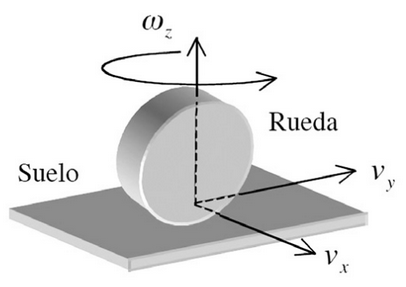
\includegraphics[width=0.35\linewidth]{rueda_modelo_cinematico}
    \caption{Vectores actuantes en una rueda}
    \label{fig:vectoresrueda}
\end{figure}

El eje $V_y$ determina el sentido normal de avance de la rueda, el eje $V_x$ indica los desplazamientos laterales y $\omega_z$ la velocidad rotacional que se produce cuando el vehículo realiza un giro.

Definimos al robot sobre el plano cartesiano, donde se establece el marco de referencia global representado por $oxy$ y el marco de referencia local del robot $o_rx_ry_r$, donde el marco de referencia local se encuentra alineado con el marco de referencia global.

\begin{figure}[H]
    \centering
    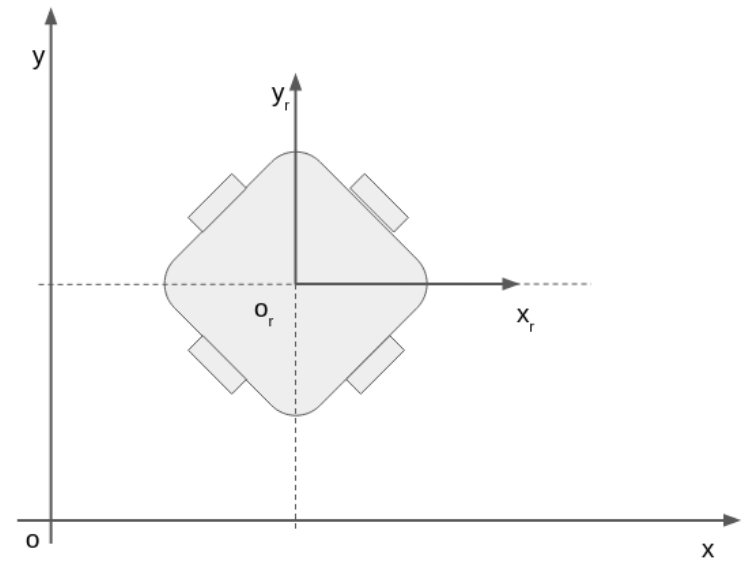
\includegraphics[width=0.5\linewidth]{robot_en_el_plano_mod_cinem}
    \caption{Marco de referencia del robot y del espacio}
    \label{fig:marcorefrobotenelplano}
\end{figure}

Además podemos representar el robot y la distribución de ruedas del siguiente modo:

\begin{figure}[H]
    \centering
    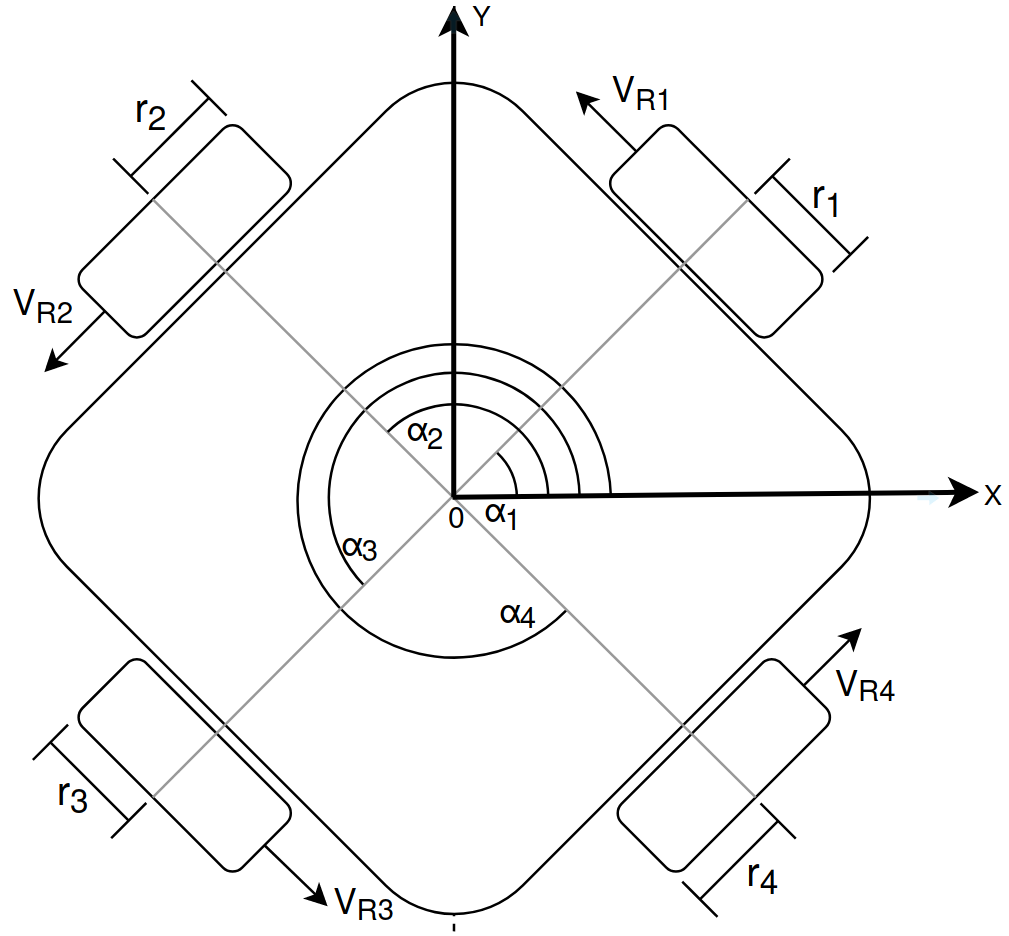
\includegraphics[width=0.5\linewidth]{images/modelo_cinematico_robot_ruedas.png}
    \caption{Descomposición de vectores del robot}
    \label{fig:vectoresrobotmodelocinem}
\end{figure}

Se establece que el angulo entre las ruedas y el cuerpo del robot es fijo y está dado por:

$$ \alpha_1 = \frac{\pi}{4} = 45^{\circ} $$
$$ \alpha_2 = \frac{3\pi}{4} = 135^{\circ} $$
$$ \alpha_3 = \frac{5\pi}{4} = 225^{\circ} $$
$$ \alpha_4 = \frac{7\pi}{4} = 315^{\circ} $$

\textbf{Cinemática Inversa} \mbox{} \vspace{8pt}

Para obtener el modelo cinemático, partimos del desarrollo de cómo afecta cada una de las ruedas al movimiento total del robot. Para ello comenzamos con la descripción del movimiento de un cuerpo rígido descrito en la Figura \ref{fig:movimientocuerporigido} \cite{islassistcontrolomni}.

$$ V_p = V_Q + W \times L $$

Utilizando el modelo de movimiento de cuerpo rígido, podemos expresar para el robot:

$$ V_{R1} = V_{01} + \omega_1 \times r_1 $$
$$ V_{R2} = V_{02} + \omega_2 \times r_2 $$
$$ V_{R3} = V_{03} + \omega_3 \times r_3 $$
$$ V_{R4} = V_{04} + \omega_4 \times r_4 $$

\begin{figure}[H]
    \centering
    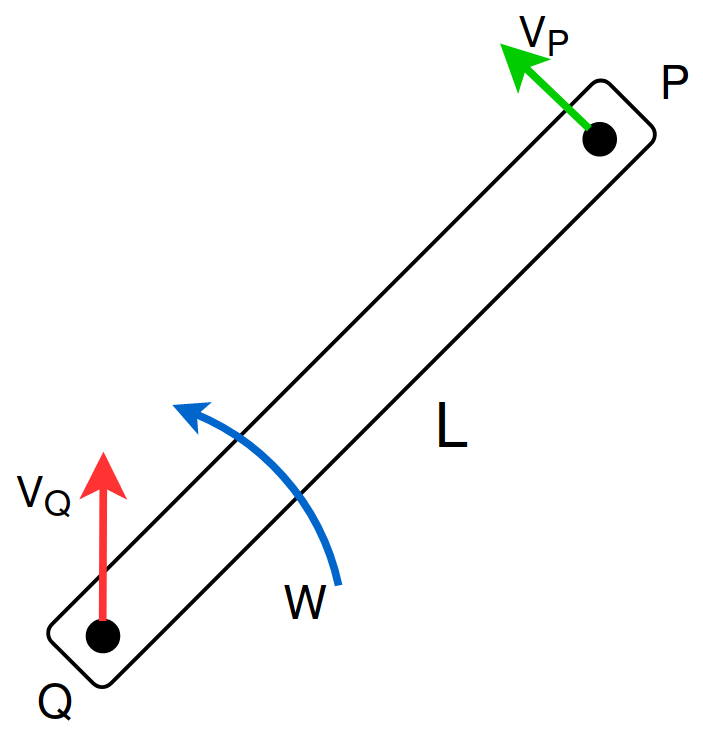
\includegraphics[width=0.3\linewidth]{images/movimiento_cuerpo_rigido.png}
    \caption{Movimiento de un cuerpo rígido}
    \label{fig:movimientocuerporigido}
\end{figure}

Se consideran $ V_{01}, V_{02}, V_{03}, V_{04} $ nulos dado que no existe deslizamiento entre las ruedas y el piso, además si todas las ruedas tienen el mismo radio, podemos expresar:

$$ V_{R1} = \omega_1 \times r $$
$$ V_{R2} = \omega_2 \times r $$
$$ V_{R3} = \omega_3 \times r $$
$$ V_{R4} = \omega_4 \times r $$

Ahora, podemos analizar el marco de referencia de la rueda respecto al marco de referencia del robot. Para ello:

\begin{figure}[H]
    \centering
    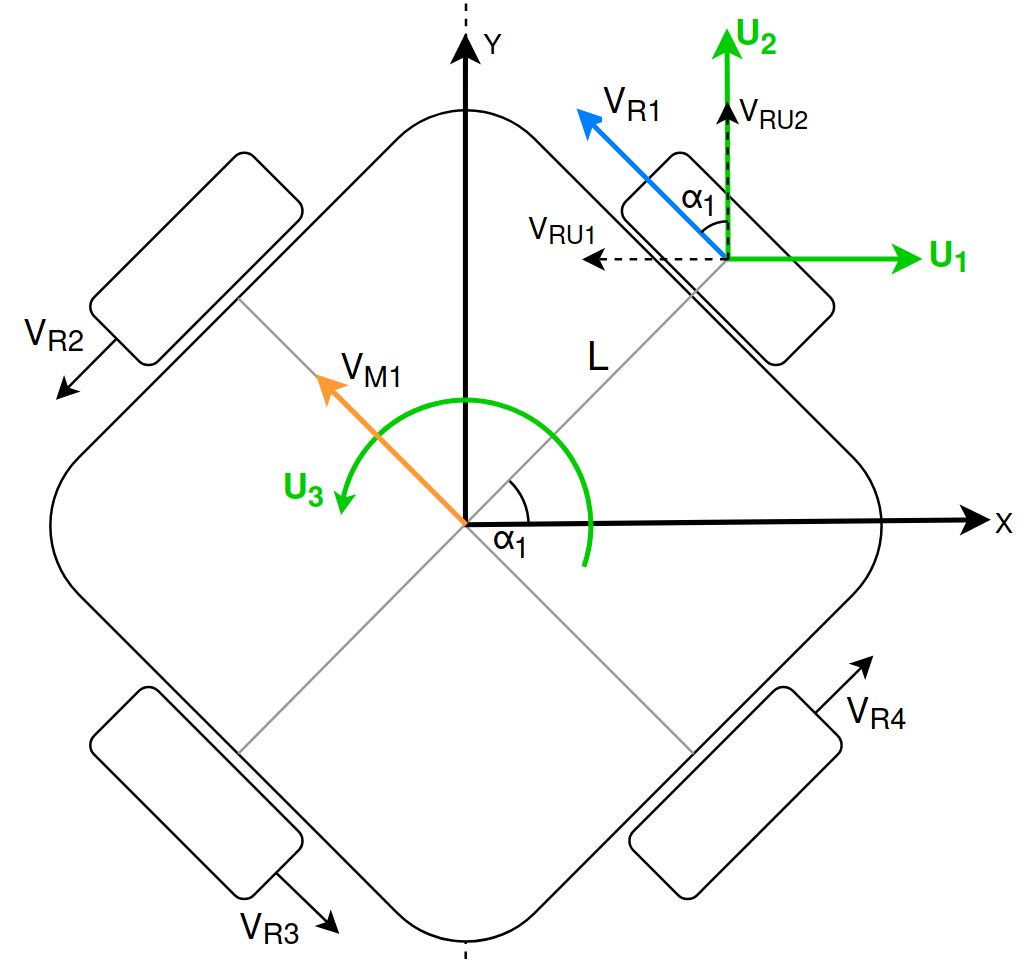
\includegraphics[width=0.6\linewidth]{images/modelo_cinematico_robot_vector.png}
    \caption{Vectores del robot en el marco de referencia local}
    \label{fig:robotmarcoreflocal}
\end{figure}

Se plantea el caso para una de las ruedas. Para obtener el vector $V_{R1}$ en base al marco de referencia denotado por $U_1$, $U_2$ y $U_3$, podemos hacer:

$$ V_{R1} = V_{M1} + U_3 \times L $$

De modo que podemos expresar $V_{M1}$ en función de $U_1$ y $U_2$:

$$ V_{M1} = V_{RU_1} + V_{RU_2} $$
$$ V_{M1} = -U_1 \cdot sen(\alpha_1) + U_2 \cdot cos(\alpha_1) $$

Obteniendo finalmente que:

$$ V_{R1} = -U_1 \cdot sen(\alpha_1) + U_2 \cdot cos(\alpha_1) + U_3 \times L $$

Al realizar el mismo procedimiento para las demás ruedas obtenemos:

$$ V_{R1} = -U_1 \cdot sen(\alpha_1) + U_2 \cdot cos(\alpha_1) + U_3 \times L $$
$$ V_{R2} = -U_1 \cdot sen(\alpha_1) + U_2 \cdot cos(\alpha_1) + U_3 \times L $$
$$ V_{R4} = -U_1 \cdot sen(\alpha_1) + U_2 \cdot cos(\alpha_1) + U_3 \times L $$
$$ V_{R3} = -U_1 \cdot sen(\alpha_1) + U_2 \cdot cos(\alpha_1) + U_3 \times L $$

Ahora bien, si $U_1$, $U_2$ y $U_3$ están alineados respecto al marco de referencia global $0XY$, podemos expresar:

$$ \begin{bmatrix} U_1 \\ U_2 \\ U_3 \end{bmatrix} = \begin{bmatrix} V_x \\ V_y \\ V_\theta \end{bmatrix} $$

Entonces ahora podemos hacer la siguiente igualdad con lo obtenido:

$$ \omega_1 \times r = -V_x \cdot sen(\alpha_1) + V_y \cdot cos(\alpha_1) + V_\theta \times L $$
$$ \omega_2 \times r = -V_x \cdot sen(\alpha_2) + V_y \cdot cos(\alpha_2) + V_\theta \times L $$
$$ \omega_3 \times r = -V_x \cdot sen(\alpha_3) + V_y \cdot cos(\alpha_3) + V_\theta \times L $$
$$ \omega_4 \times r = -V_x \cdot sen(\alpha_4) + V_y \cdot cos(\alpha_4) + V_\theta \times L $$

Originalmente partimos de que necesitamos una matriz de conversión de modo que podamos obtener las velocidades de las ruedas en base a un vector dado, donde la entrada es $V_x, V_y$ expresadas en $[m/seg]$ y $V_\theta$ expresada en $[RPM]$. Por otra parte, la salida $\omega_n$ se determina en $[rad/seg]$:

$$ \begin{bmatrix} w_1 \\ w_2 \\ w_3 \\ w_4 \\ \end{bmatrix} = IK \cdot \begin{bmatrix} V_x \\ V_y \\ V_\theta \\ \end{bmatrix} $$

Con las expresiones anteriores, obtenemos que la matriz cinemática inversa se puede expresar como:

$$ IK = 
    \frac{1}{r}
    \cdot
    \begin{bmatrix}
        {-sen(\alpha_1)} & {cos(\alpha_1)} & L \\
        {-sen(\alpha_2)} & {cos(\alpha_2)} & L \\
        {-sen(\alpha_3)} & {cos(\alpha_3)} & L \\
        {-sen(\alpha_4)} & {cos(\alpha_4)} & L \\
    \end{bmatrix} $$

De modo que podemos expresar la ecuación para obtener las velocidades de las ruedas expresadas en $[rad/seg]$ como se muestra debajo.

$$ \begin{bmatrix} w_1 \\ w_2 \\ w_3 \\ w_4 \\ \end{bmatrix} = \frac{1}{r} \cdot \begin{bmatrix}
    {-sen(\frac{\pi}{4})} & {cos( \frac{\pi}{4})} & L \\
    {-sen(\frac{3\pi}{4})} & {cos(\frac{3\pi}{4})} & L \\
    {-sen(\frac{5\pi}{4})} & {cos(\frac{5\pi}{4})} & L \\
    {-sen(\frac{7\pi}{4})} & {cos(\frac{7\pi}{4})} & L \\
\end{bmatrix} \cdot
\begin{bmatrix} V_x \\ V_y \\ V_\theta \\ \end{bmatrix} $$

Dado que las MotorTask de cada una de las ruedas recibe el setpoint en $[RPM]$, debemos hacer una conversión a esa unidad. Por lo que planteamos una matriz que convierta los valores de las dos primeras columnas de la matriz cinemática, que son los coeficientes que nos interesa convertir a $[RPM]$, dado que los de la última columna ya están expresados en esa unidad.

$$ \begin{bmatrix} w_1 \\ w_2 \\ w_3 \\ w_4 \\ \end{bmatrix} =
    \frac{1}{r}
    \cdot
    \begin{bmatrix}
        {-sen(\frac{\pi}{4})} & {cos( \frac{\pi}{4})} & L \\
        {-sen(\frac{3\pi}{4})} & {cos(\frac{3\pi}{4})} & L \\
        {-sen(\frac{5\pi}{4})} & {cos(\frac{5\pi}{4})} & L \\
        {-sen(\frac{7\pi}{4})} & {cos(\frac{7\pi}{4})} & L \\
    \end{bmatrix}
    \cdot
    \begin{bmatrix}
        {\frac{60}{2 \pi}} & {0} & {0} \\
        {0} & {\frac{60}{2 \pi}} & {0} \\
        {0} & {0} & {1}                \\
    \end{bmatrix}
    \cdot
    \begin{bmatrix} V_x \\ V_y \\ V_\theta \\ \end{bmatrix} $$


\textbf{Cinemática Directa} \mbox{} \vspace{8pt}

Para lograr el control del robot sobre el plano es necesario hacer una comparación entre el vector de movimiento deseado y un vector de movimiento inferido en base a la medición de la velocidad de las ruedas, de modo que se cierra el lazo de control. El error existente entre el vector real y el deseado es debido a que los motores no establecen las RPM inmediatamente por cuestiones de inercia e imperfecciones en el terreno.

Para obtener el vector de velocidad lineal real que efectivamente realiza el robot, hacemos uso de las mediciones de velocidad angular en cada rueda y se ingresan a la ecuación cinemática directa. Esta matriz se obtiene a partir de la pseudoinversa de la matriz cinemática inversa. \cite{islassistcontrolomni}

De modo que, en primer lugar obtenemos la matriz de conversión que nos permite obtener el vector lineal en base a las velocidades de las ruedas expresadas en $[rad/seg]$:

$$ \begin{bmatrix} V_x \\ V_y \\ V_\theta \\ \end{bmatrix} = DK \cdot \begin{bmatrix} w_1 \\ w_2 \\ w_3 \\ w_4 \\ \end{bmatrix} $$

Luego, al realizar pseudoinversa de la matriz $IK$:

$$  DK = 
    r
    \cdot 
    \begin{bmatrix}
        {\frac{-sen(\alpha_1)}{2}} & {\frac{-sen(\alpha_2)}{2}} & {\frac{-sen(\alpha_3)}{2}} & {\frac{-sen(\alpha_4)}{2}} \\
        {\frac{cos(\alpha_1)}{2}}  & {\frac{cos(\alpha_2)}{2}}  & {\frac{cos(\alpha_3)}{2}}  & {\frac{cos(\alpha_4)}{2}}  \\
        {\frac{1}{4L}}  & {\frac{1}{4L}}  & {\frac{1}{4L}}  & {\frac{1}{4L}}  \\
    \end{bmatrix} $$

Por lo que obtenemos la siguiente expresión para obtener el vector de movimiento del robot dependiendo las velocidades de las ruedas:

$$ \begin{bmatrix} V_x \\ V_y \\ V_\theta \\ \end{bmatrix} = 
    r
    \cdot 
    \begin{bmatrix}
        {\frac{-sen(\alpha_1)}{2}} & {\frac{-sen(\alpha_2)}{2}} & {\frac{-sen(\alpha_3)}{2}} & {\frac{-sen(\alpha_4)}{2}} \\
        {\frac{cos(\alpha_1)}{2}}  & {\frac{cos(\alpha_2)}{2}}  & {\frac{cos(\alpha_3)}{2}}  & {\frac{cos(\alpha_4)}{2}}  \\
        {\frac{1}{4L}}  & {\frac{1}{4L}}  & {\frac{1}{4L}}  & {\frac{1}{4L}}  \\
    \end{bmatrix}
    \cdot
    \begin{bmatrix} w_1 \\ w_2 \\ w_3 \\ w_4 \\ \end{bmatrix} $$

Esta expresión toma las velocidades angulares de las ruedas en $[rad/seg]$, por lo que necesitamos convertir la entrada para que pueda ser $[RPM]$. Para ello planteamos una matriz que solo convierta los valores de las dos primeras filas, que son los coeficientes que nos interesa convertir a $[RPM]$, dado que los de la última fila ya están expresados en esa unidad.

$$ \begin{bmatrix} V_x \\ V_y \\ V_\theta \\ \end{bmatrix} = 
    r
    \cdot 
    \begin{bmatrix}
        {\frac{2\pi}{60}} & {0} & {0}  \\
        {0} & {\frac{2\pi}{60}} & {0} \\
        {0} & {0} & {1} \\
    \end{bmatrix}
    \cdot
    \begin{bmatrix}
        {\frac{-sen(\alpha_1)}{2}} & {\frac{-sen(\alpha_2)}{2}} & {\frac{-sen(\alpha_3)}{2}} & {\frac{-sen(\alpha_4)}{2}} \\
        {\frac{cos(\alpha_1)}{2}}  & {\frac{cos(\alpha_2)}{2}}  & {\frac{cos(\alpha_3)}{2}}  & {\frac{cos(\alpha_4)}{2}}  \\
        {\frac{1}{4L}}  & {\frac{1}{4L}}  & {\frac{1}{4L}}  & {\frac{1}{4L}}  \\
    \end{bmatrix}
    \cdot
    \begin{bmatrix} w_1 \\ w_2 \\ w_3 \\ w_4 \\ \end{bmatrix} $$


\paragraph{Implementación} \mbox{} \vspace{8pt}

Para la implementación se propuso que el modelo cinemático sea contenido dentro de la MasterTask dado que es quien recibe el feedback de todas las tareas MotorTask y conoce el estado actual de cada uno de los motores. Un diagrama de secuencia se detalla más adelante en este capítulo.

\begin{figure}[H]
    \centering
    \hspace*{-0.75cm}
    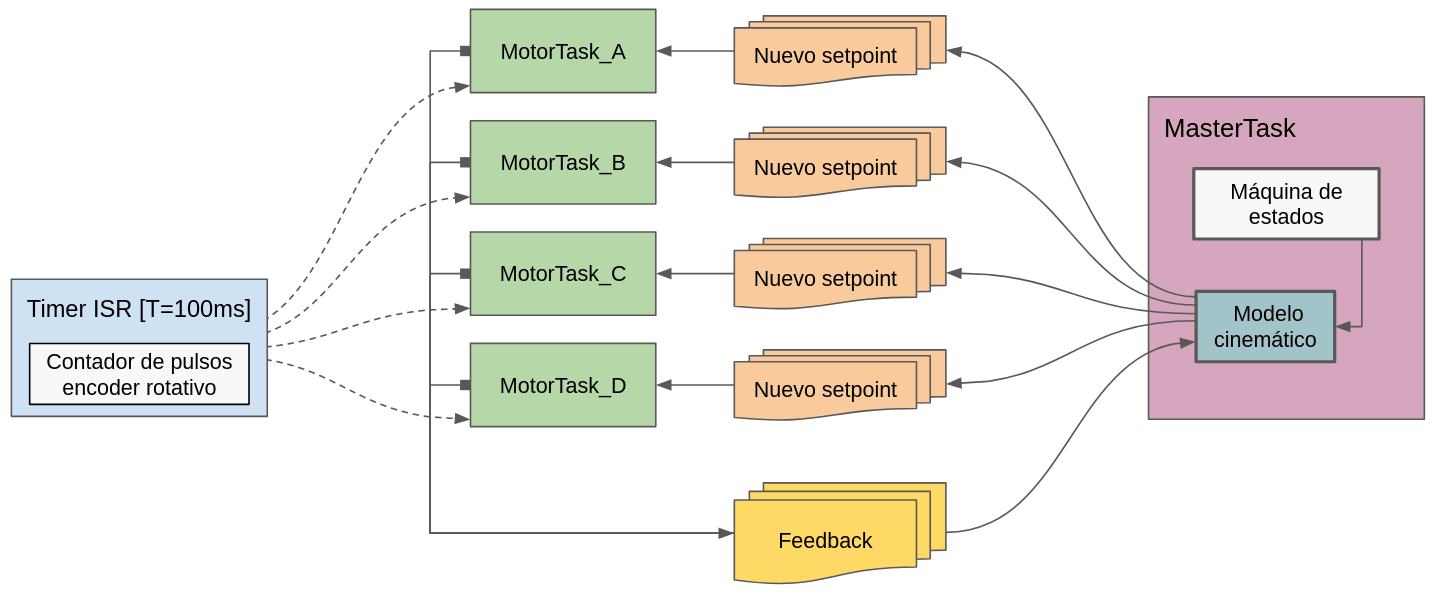
\includegraphics[width=1.1\linewidth]{images/diag_comp_esp32_modelo_cinem.png}
    \caption{Estructura de control de los motores con el Modelo Cinemático}
    \label{fig:diagcomponentesp32modelocinem}
\end{figure}
